\documentclass[a4paper,12pt]{article}
\usepackage[english]{babel}
\usepackage{graphicx}
\graphicspath{ {images/} }
\usepackage[font=it,labelfont=bf]{caption}
\usepackage{algorithm}
\usepackage{algpseudocode}
\usepackage{varwidth}
\usepackage{amsmath}
\usepackage{amsthm}
\usepackage{subcaption}
\usepackage{float}
\usepackage{titlesec}
\usepackage{cleveref}
\usepackage{cite}
\usepackage{url}
\usepackage{harvard}
\usepackage{thm-restate}
\usepackage[space]{grffile}

\citationmode{abbr}


\linespread{1.3}

\captionsetup[subfigure]{subrefformat=simple,labelformat=simple}
\renewcommand\thesubfigure{(\alph{subfigure})}

\setcounter{secnumdepth}{4}
\newcommand{\myparagraph}[1]{\paragraph*{#1}\mbox{}\\}

\newtheorem{theorem}{Theorem}[section]
\newtheorem{lemma}[theorem]{Lemma}
\newtheorem{defin}{Definition}
\newtheorem*{rquestion}{Question}
\newtheorem{subquestion}{Sub-Question}
\newcommand{\mydef}[3]{
\begin{defin}
\textsc{#1}

Given: #2

Question: #3
\end{defin}}

\newcommand{\bigO}[1]{$\mathcal{O}$($#1$)}
\newcommand{\bigOs}[1]{$\mathcal{O^*}$($#1$)}
\newcommand{\NP}{$\mathcal{NP}$}
\newcommand{\acco}[1]{\{ #1 \}}

\newcommand{\vecarr}[3]{\overset{#2}{\overrightarrow{#1}}}

%Door deze regel springt de eerste regel van
%elke alinea niet meer steeds een stukje in.
%\setlength{\parskip}{\baselineskip}
%Door deze regel wordt tussen de alinea's steeds
%een regel overgeslagen.

%\setlength{\columnseprule}{1pt}
%\def\columnseprulecolor{\color{blue}}

\newcommand{\algorithmicbreak}{\textbf{break}}
\newcommand{\Break}{\State \algorithmicbreak}



\begin{document}
\title{Simulation and Optimisation of Offshore Renewable Energy Arrays for Minimal Life-Cycle Costs}
\author{Robin Kuipers \\[1cm] Supervisors: \\ Kerem Akartunali \\ Euan Barlow\\[2cm] University of Strathclyde \\ Strathclyde Business School \\ {\small Glasgow, Scotland}}
\date{January, 2020}

\maketitle

\pagebreak

\begin{abstract}
This report aims to give a detailed overview of the research progress I made between March 2018 and September 2019, the first year and a bit of this PhD project into logistical decisions regarding offshore wind farms. It will explain the research subject, give an overview of the relevant literature I've read and the limitations of the current research. Furthermore, it will discuss the work I've done on a simulation tool, to be used for later research. Finally, the next steps and ultimate goals of this project are described. 
\end{abstract}

\pagebreak

\tableofcontents

\pagebreak

\section{Introduction} \label{s:intro}
%TODO: Add refs for `several years' and `30 years' claims
Over the past year, I have been researching logistics related to offshore windfarm projects; the installation, maintenance, and decommissioning of windfarms in various seas and oceans, primarily the North Sea. The installation and decommissioning projects can often take up to several years, and the lifespan of such farms is about 30 years, over which maintenance has to be done. For these projects, expensive vessels have to be used, the rent of which is often upwards of \pounds 100.000 per day \cite{barlow2014support}, hence a project with multiple vessels over many months can cost upwards of \pounds 100 million \cite{kaiser2010offshore}. Therefore, even small improvements to the schedules can save significant amounts of money.

Because of this, I expected a lot of research in this area had already been conducted, but this turned out to be less the case than I would have expected. Most research is fairly recent, and there are significant literature gaps. The primary obstacle in this logistics problem which separates it from more traditional logistics problems is the high degree of nondeterministic factors, mainly related to the weather conditions. These projects take place on open sea, where weather can often be rougher than on land. In addition, the high-tech vessels are performing operations on large industrial constructions, hence there is a limited range of allowed wind speeds and wave heights. Something else which can further limit possible schedules is the inflexibility involved in vessel rental, since vessels of the required calibre cannot be rented on short notice, and often need to be rented for at least some minimum amount of time \cite{kerkhove2017optimised}, so adaptive in-the-moment scheduling is impossible and we cannot simply wait for an expected period of good weather based on real-time data to rent the vessels; if we expected some period to have good weather but this turns out not to be the case, we will often have the vessels rented but unusable. This means the problem has a lot of nondeterministic factors which have a large impact; factors which any good solution approach will have to take into account. 

In this report I will talk about my progress and what I have learned over the past year. First, in \Cref{s:project}, I will explain the examined problem in more detail, and introduce the goals of this research project. After that, in \Cref{s:meth} the methods I intend to use (simulation and optimisation) will be discussed in detail. In \Cref{s:lit}, I will recount the reading I have done so far, which was the main focus of my work over the past year. This will include both research on this specific project, and research in the more general fields of (stochastic) scheduling. These two sections on methods and literature will be the main focus of the report, as it was the main focus of my work so far. In addition to reading up on the state of the current research, I have also started building a Simulation tool for this problem, which I will discuss in \Cref{s:sim}. My other activities, such as some courses about research that I followed, are summarised in \Cref{s:otact}. Finally, I will summarise my current standing and plans for future work in \Cref{s:concl}. 

\pagebreak

\section{The project} \label{s:project}
In this section I will describe my research project in more detail, and discuss the questions I aim to answer by the end of it. This should provide sufficient context for the rest of the report. 

My project is about optimising all sorts of logistical decisions regarding offshore energy sites, primarily windfarms. This includes supply chains, routing, design of the windfarm, and scheduling of the operations to be done on the windfarm. The latter is where my primary focus lies, and what the majority of this report will be about. 

\subsection{Logistical decisions on offshore windfarms} \label{ss:logdec}
The type of offshore windfarm (OWF) this research project will focus on is described in \cite{barlow2018mixed}. A typical windfarm of this type will have two types of structures: Wind Turbine Generators (WTGs) and Offshore Substation Platforms (OSPs). The WTGs are the actual turbines generating energy, and the OSPs are hubs where the power generated in the WTGs is gathered and transformed before being transported to shore. Between these structures are many cables, connecting the WTGs to the OSPs, generally with a number of sets of WTGs connected serially. Then from each OSP there are specialized cables back to shore. A typical OWF currently in development might have upwards of 100 WTGs and 2 OSPs \cite{ruk2017}. 

The life-cycle of an OWF can be broken up into three phases: installation, maintenance and decommissioning. Installation and decommissioning are similar in structure; a fixed set of tasks needs to be completed in a cost-effective way. The primary difference is the reversed order of the tasks. For each of the structures there is a set of tasks that need to be completed in series for each individual structure, such as (for installation): preparing the sea surface, laying the foundation, installing the structure and laying the cables (each of these tasks may be split into more tasks such as loading, transport and installation) \cite{kerkhove2017optimised}. Within the group of tasks for a structure, most tasks will have to be performed in a specific order, while the tasks for separate structures can be completed in any order. This is essential for some of the more sophisticated objective functions used in the literature; if one OSP and a set of WTGs connected to it are active, they can start generating power while the rest of the wind farm is still under construction \cite{barlow2017using}. This is often a contractual requirement imposed by the government, and it would also mean the farm starts making money significantly earlier, and can therefore have significant impacts on desired schedules. This can lead to contractually or legally enforced deadlines for certain milestones, like 10\% or 50\% of the WTGs being operational.

The structure of maintenance projects is completely different. The set of tasks in not fixed, and ideally maintenance would only be performed right before an asset was about to fail. However, this is impossible to predict, and due to long lead up times of renting maintenance vessels waiting for an asset to fail will cause long periods of downtime. Scheduling maintenance has to be done significantly in advance. It is also costly, meaning maintenance trips which would have been unnecessary are undesirable as well. These two factors mean an efficient maintenance policy needs to find a balance between not spending too much on maintenance, and maintaining high uptime on the structures of the site (especially OSPs being offline can lead to massive losses in profit). 

%TODO: Possibly add something about subjectivity, and the goal not being finding a `perfect' schedule but a number of candidate schedules
The stochastic nature of the project also comes with various challenges. Naively one would perhaps go for the schedule with the lowest expected cost or the earlier expected end time. But the specific goal depends on the wishes of the executing company and project details. For example, a company may want at least 95\% certainty that the project is complete (or complete up to some milestone) by a given deadline, or some certainty that the costs do not exceed a given threshold. Therefore the probability distribution of the cost and duration of a resulting schedule are important to determining the value of that schedule. Additionally it is worth noting that while the end time of a schedule and the cost are strongly related, there are scenarios in which it is more profitable to halt the operations for a number of months, especially the winter months where there will be more days with weather too extreme to perform operations in. While this break would obviously postpone the total completion of the schedule, not having to pay rent for vessels over these months in which they cannot perform optimally might lead to a higher net profit over all, especially if a part of the windfarm is already operational and generating energy over these months. In this way, schedules need to be determined on various levels; there are day-to-day decisions, and much larger decisions regarding operational periods. 

%TODO: For the cites, look at sources and where they got it from; citing directly leads me to more (varied) sources

\subsection{This research project} \label{ss:objs}
The primary goal of this project is to look at the entire life-cycle of OWFs, and how decisions at different points in this life-cycle impact the situation at other points in time. Specifically I aim to use both optimisation and simulation to provide insight into logistical decisions, primarily scheduling, but potentially also layout of the site and the routing on it. The latter two are very challenging subjects on their own, and I will likely only run simplistic experiments with them, to see whether looking at a full life-cycle gives any insights on its own. Therefore the primary focus will lie on scheduling, specifically scheduling that considers the entire life-cycle. 

Over the past year, I have spent most of my time reading up on the subject, both the methods and the challenges of offshore projects. This literature is summed up in \Cref{s:lit}. Additionally I have been laying the groundwork for a simulator which I am planning to turn into a tool for support on the logistical decisions described previously. Details on this tool are given in \Cref{s:sim}.

\bigskip

The primary research question is:

\begin{restatable}{rquestion}{rquest}
Can considering the entirety of the life-cycle of an Offshore Wind Farm, and how each of the phases interact, improve logistical decision making on these projects?
\label{rquest}
\end{restatable}

The primary motivation for this objective is that in the literature the three phases of the life-cycle are each treated separately, while they might heavily influence each other. There is a large amount of research done on the maintenance projects, and quite a bit on installation projects as well, while decommissioning projects are less well researched. However no research was found considering all three phases simultaneously. Treating these phases as separate makes them more manageable, but some insight about how they influence each other is also valuable. There are two primary ways in which these phases interact; some partially take place at the same time and share resources, and any phase affect any phase after it. 

For the first type of interaction it is important to consider that the maintenance phase overlaps with both other phases for some amount of time. Once the first set of wind turbines has been fully installed they start producing energy and might require maintenance, while the rest of the turbines are still being installed. It may be beneficial to use the same vessels to install the remaining wind turbines and perform maintenance, or have separate vessels that still use the same ports and have to consider the routing of the installation vessels. The same thing happens at the end of the life cycle; when decommission starts specific wind turbines are decommissioned while others continue to produce energy. 

%TODO: Cite someone regarding the possible explanation for low decomisison research
The second type of interaction has to do with any event in the life-cycle of a wind turbine (or the entire farm) affecting all events that come after it, regardless of which phase these events are part of. The order in which the turbines are installed determines their age, and affects their expected failure rate when maintenance starts on them. In a more extensive way, any failures and repairs during the maintenance phase influence which wind turbines are most likely to fail again, and therefore which are most efficient to decommission first. With that in mind it is clear that decommission is the phase which relies most heavily on what happens before it, which may be one of the reasons why it has been studied less than the other two phases. This type of interaction means simulating the early stages of the life-cycle of the windfarm might lead to more accurate and realistic knowledge to base decisions in the later stages of the life-cycle on. For example, basing the order in which turbines are decommissioned on their actual history of failures and reparations is expected to lead to better result than a predetermined arbitrary order. 

This interaction works in the other direction as well. Instead of the history of the windfarm influencing decisions near the end of the life-cycle, the future of the windfarm can also influence early decisions. For example, if we compare two installation schedules and base our choice solely on a measurement done during the installation phase (such as the date the installation finishes, or the cost at time of finishing) this could potentially lead to another option than if we look at the entire life-cycle. Non-operational periods are times of the year (usually winter months) in which no installation operations are performed on the site due to the severe weather conditions. Using periods like this leads to larger age differences between turbines, which could influence the maintenance and decommission phases. This effect cannot be fully measured unless the entire life-cycle is considered, and knowing the effect could influence decisions regarding the non-operational periods. 

Through these interactions we state three sub-questions for the above research question:

\begin{restatable}{subquestion}{sqa}
\label{sqa}
Can considering how phases in the life-cycle of a windfarm overlap and share resources improve logistical decision making on these projects?
\end{restatable}

\begin{restatable}{subquestion}{sqb}
\label{sqb}
Can simulating the entire life-cycle of a windfarm provide useful data to base logistical decisions on in the later phases of these projects?
\end{restatable}

\begin{restatable}{subquestion}{sqc}
\label{sqc}
Can considering the long-term effects of logistical decisions early on in the life-cycle of a windfarm improve these decisions? 
\end{restatable}

While the latter two questions seem similar, they approach the same phenomenon from different perspectives. This will likely lead to different techniques and models being used to answer them. 

\pagebreak

\section{Methods} \label{s:meth}
The most commonly used methods for projects such as this, which are also the methods I plan to use, will be discussed in this section. These methods are Simulation and Optimisation, and they can be used seperately or together. I will discuss both the basics of the methods, as well as how they apply to this research. 

\subsection{Simulation} \label{ss:sim}
Simulation, especially Discrete Event Simulation, is a very broadly used method in computational analysis \cite{law2000simulation,robinson2010conceptual}. A simulation effectively walks through every step in a process, letting all random variables take on a specific value. A single run of a simulation like this is not very useful in itself, but if a lot of runs are done (with different specific values for the random variables in every run) it can lead to a better understanding and evaluation of the situation. For example, when a train timetable is made possible delays need to be kept in mind. Delays can cause disturbances and can potentially cause chain reactions when it does not leave a certain platform before the next train is supposed to arrive there. It is very difficult to analyse this process analytically, which makes it very difficult to evaluate a proposed timetable analytically. However if a timetable is used in 1000 runs of a simulation, we can have some idea about how common these disturbances are. Simulations are very suited to help in situations like this, where there are a lot of random variables and events that depend on each other (a platform needs to be empty for the next train to arrive). 

If we look at the offshore projects discussed in my research, the insights we can gain from this are not merely an expected (average) duration of a project. For example, a confidence interval for the costs of the project or the probability a certain task will be completed before a set time can also be examined. However, simulation for these offshore projects heavily relies on the weather model and data. Simulation is primarily about examining the effects of uncertainty, and the weather is a major source of uncertainty, our choice of how to model the weather and which data to use for it is crucial. 

\subsubsection{Reliance on weather data} \label{sss:weather}
If the weather data is limited in precision or amount of data available, the applicability of the simulation results in turn will also be limited. A simulation as detailed as we would like for this type of project would have timesteps in the range of 15 minutes to an hour. A lot of weather data has much larger timesteps, often of several hours. There are methods to interpolate between weather data points, but this tends to not be very precise as there are a lot of factors to take into account. The most important measures of the weather are wind speed and wave height, as by these measures the usability of the vessels can be determined. In order for this data to be realistic, the two measures have to be correlated, as well as have autocorrelation over time. Having those values be realistically interpolated between two measured points is a difficult task, and something we will have to figure out a way to realistically handle for future research.

The amount of data available is also a common problem. A major reason for this is the natural change of weather depending on the time of year. Generally, a year would be split up in sections, for example the four seasons or the twelve months. Intuitively this makes a lot of sense; if we want to model the weather in January data from July is irrelevant for this. But the consequence is the sheer amount of time it takes to collect accurate data for each time period; if we want 300 days of data for the month of April, we need data collected over the span of 10 years. In addition, the conditions of the location the data is gathered from have to be similar to the location of the OWF. An important parameter for this is the distance to the shore, but there are more factors which play a part. 

A method to handle these drawbacks of the weather data is to not use raw data, but analyse the periodic characteristics of the change of both wind and wave states. Using these characteristics, one can generate weather data by drawing a random real data point within the desired time period, and extrapolating the data from there using the found characteristics. This is used frequently in the literature, and has been shown to have a good potential for stochastic simulations. 

Another method we are planning to explore relates more to robust optimisation. It might not be necessary to have a large number of simulations for all possible weather conditions. If, for each time period, we create a range of possible wind and wave states (including the extreme cases from the data) and run simulations for a set of (realistic) combinations of them we could aim to make a robust schedule that performs well within even the most extreme weather scenarios without having too many simulations to run. The drawback of this robust approach is a schedule that performs well in 99\% of weather cases might be discarded for the most extreme 1\% of cases. This can however be reduced by carefully selecting the data to use for the simulations, or allowing a certain number of bad scenarios (especially if the weather causing it is very rare).

%TODO: Citations?

\subsection{Optimisation} \label{ss:opt}
Optimisation, in particular through (mixed-)integer programming, is an essential tool in problems like this, and is used extensively in the literature \cite{nemhauser1999integer,lee2011mixed}. This is effectively the practice of choosing some decision variables to be decided, an objective function based on them to optimise, and the restrictions on the variables. After this is done a computer algorithm can find the allowed values of the decision variables for which the value of the objective function is optimal. 

An example based on OWF planning would be a binary decision variable $x_{ij}$ for each combination of task $i$ and vessel $j$. If $x_{ij}$ is 1 then task $i$ is assigned to vessel $j$ and otherwise $x_{ij}$ is 0. A number of basic restrictions on this would be that the values $x_{ij}$ can only take the values 0 and 1, that each task is assigned to exactly 1 vessel, and possibly that each vessel can only be assigned certain types of tasks (a crew transport vessel cannot be assigned operational tasks). An example objective function could be one that sums up the total expected task duration for each vessel (by summing up the expected durations of all tasks assigned to it) and tries to find values for the $x_{ij}$ variables such that the highest value of this sum over all values in minimised (such that tasks are distributed as evenly as possible). 

There are a number of different categories of this method, based on the possible values the decision variables can take and how the value of the objective function might change depending on them. Linear programming (where the relation between each variable and the value of the objective function is linear) and integer programming (where the decision variables can only take integer values) are generally preferred as other forms are computationally much more complex to solve, and are therefore restricted in size in order to be solved in feasible time. However, many problems require these more complex variations.

Even linear and integer programming models computationally complex to solve, hence many methods are used to reduce to complexity of the models. There are standard techniques like Lagrangian relaxation \cite{fisher1981lagrangian} and column generation \cite{barnhart1998branch}, but there are more specific methods used as well. The primary way this is done is by limiting the scope of individual optimisation problems (not necessarily the research), by splitting up the research and using multi-level optimisation models, or using simulation for certain parts of it. 

Another method has been discussed before already; robust optimisation. As with simulation, this reduces the number of considered inputs (primarily weather states, but also task duration which is sometimes stochastic) by only considering certain constructed uncertainty sets. This strongly reduces the number of situations considered in the optimisation. Literature which uses and examines this method is discussed in \Cref{ss:stoch}. 

\bigskip

There are different froms of optimisation than computational programming. The most prominent are heuristic methods, such as local search. Heuristics are powerful when dealing with large problems like this, as finding an exact global optimum will usually take an infeasibly long time. A benefit of local search is that reasonably good results can often be found fairly quick, but this is connected to the main drawback of local search; it can often be difficult to get out of local optima. However, there is a lot of literature on local search and other heuristics and many variants designed to reduce its drawbacks. 

Alternatively, evolutionary algorithms have been used for deterministic scheduling problems such as machine learning \cite{dorndorf1995evolution}. A good explanation of this technique for scheduling is given in \cite{cotta2007memetic}. While this technique seems to be fairly common in deterministic scheduling, not much research could be found in an uncertain setting. The exception is \cite{sevaux2002genetic} as discussed in \Cref{ss:stoch}. This research, although seemingly brief, gives quality results. Since there is no clear reason why evolutionary algorithms couldn't work well within an uncertain setting, this is a potential method to explore in the future. 

\subsection{Combining Simulation and Optimisation} \label{ss:simopt}
%TODO: Double check if I don't want to say more about my method of combining opt and sim should be explained more here (based on whats discussed later and the research questions and stuff
When optimisation is to be performed within nondeterministic environments, it is often combined with simulation, such as in \cite{de2003integrating} and \cite{bard2015integrating}. A primary reason for this, and why I plan on using this too, is that simulation is a very effective way to analyse large-scale schedules subject to uncertain conditions. The optimisation and simulation model can be integrated by using the simulation to evaluate a schedule proposed by the optimisation model. This can often give more accurate results than using a simplistic objective function. The simulation model can then return an appropriate metric regarding the quality of the schedule, such as makespan or total cost, and the optimisation model can aim to improve from there. In theory this integration can even be extended; the simulation model can determine metrics relating to specific subsets of tasks, and potentially the optimisation model can use this extensive data to make more effective optimisations. For example, the set of tasks may have several types of tasks or distinct phases separated by milestone tasks. If a certain type or phase of tasks has a high ratio of delayed tasks, this might be a good part of the schedule to focus on for future changes. 

The exact manner in which simulation and optimisation are combined depends on the project and individual models, but the above technique is very promising for offshore construction projects, and similar to the model used in \cite{kerkhove2017optimised}. 

\pagebreak

\section{Literature} \label{s:lit}
In this section I will give an overview of the literature I have read to-date for this research. I will discuss some actual attempts to produce a schedule for the installation problem in \Cref{ss:sched}, and research on the maintenance of the site will be shown in \Cref{ss:maint}. Other research related to offshore projects is shown in \Cref{ss:offsh}. Some other studies to do with uncertain scheduling will be highlighted in \Cref{ss:stoch}.  

\subsection{Scheduling the installation} \label{ss:sched}
Here I will take an in-depth look into two papers that use comparable methods to look at the issue of producing an efficient schedule, and discuss their strengths, weaknesses, and difference.

\bigskip

In \cite{barlow2018mixed} a mixed-method approach is used. They identify the strengths and weaknesses of both simulation and optimisation, and aim to use the methods together in a way that utilises the strength of each. First a simulation is used to determine some amount of delay before starting the project, as this can have sizeable impact on the total duration of the project. Then, a mathematical programming model is used to construct a schedule from this starting point. The output of that optimisation model is then used in the simulation to give a view of the overall costs under uncertain circumstances. 

For the simulation a synthetic weather time-series model is used. This weather model is described in full in \cite{dinwoodie2014operational} , and uses a correlated auto-regression model which identifies underlying trends in the data and aims to predict future behaviour over time. This seems to be a fitting and sophisticated model. In the optimisation model a more simplistic model is used. Tasks are given a minimal duration $d_{i, min}$ and a maximum increase $d_{i, inc}$ of that duration. The realised duration is given by $d_{i,  min} + z_i d_{i, inc}$ for some $0 \leq z_i \leq 1$. The programming model has two levels; the outer model maximises $\sum_i z_i \leq \Gamma$ for some given limit $\Gamma$. The inner model then uses the fixed values $z_i$ to set the start times of each task in accordance with their deadlines and precedence relations. 

In effect, a $\Gamma$ is chosen to represent a certain percentage of tasks taking their maximum duration. For example, if there are 200 tasks and 10\% of them can take the maximum duration, $\Gamma$ is set to 20, and this can either result in 20 tasks taking their maximum duration with all other tasks being completed in the minimum duration, or every task taking 10\% of its maximum extra time ($d_{i, inc}$). 

\bigskip

I have a number of criticisms about this research, which I will now discuss.

The way delay is modelled in the optimisation model considers delays independent, while in practice there are clear patterns. Often multiple vessels are used, meaning multiple tasks are scheduled for the same time. If one of the tasks is delayed due to the weather, any other tasks scheduled for that time will have to be done under the same weather conditions and are therefore more likely to be delayed. The same holds for two tasks done concecutively by the same vessel, as the weather conditions will be similar for these tasks. 
Another criticism of the way delays are modelled tasks have a maximum amount of time they could be delayed, but other papers in this field (including the one discussed in the latter half of this section) mention than many tasks cannot be performed at all under certain weather conditions. This is structurally different behaviour from a task simply taking longer, as it may delay any of that type of task for hours or even days. This behaviour is still included in the simulation, so it is tested for when evalutating the quality of a schedule. However it seems the schedules could be improved if this behaviour was considered in the optimisation model as well. 

An additional criticism to make this research more applicable is the objective function used in optimisation. The makespan of the longest path of the schedule is minimised, but a company doing the installation will often be more interested in the total cost of a schedule. This is clearly very related to the makespan, but can differ if certain vessels are used for longer than others, and when parts of the OWF can become active (and generate profit) earlier. Early completion of sections of the windfarm are currently treated as certain milestones to reach, but when using the monetary value of the project in the objective function the actual financial benefits of early completion take effect. The common practice of discounting the cost and value future spending and profit could also be incorporated in this to more accurately represent the interests of the company. It seems like more research into this could therefore be beneficial. 

Finally the strengths of the simulation could be utilized more. In the research presented, a start date is determined at the start and this is then used in the optimisation and for the rest of the research. However in determining a start date a very rudimentary schedule is used. Optimal schedules starting in each month could be explored more, as well as pausing the operations after they started. For example, if the winter months turn out to be very difficult and slow to work in, the project could be paused over several months, over which no rent for the vessel would have to be payed. This would seem to be particularly effective if a subset of the WTGs could be operational before pausing, as they would generate energy (and revenue) during winter. These periods of time are called non-operational periods, and are sometimes used in large projects such as these.  

\bigskip

A different model is designed in \cite{kerkhove2017optimised}. It uses similar methods as used in \cite{barlow2018mixed}, namely a mixed-method of optimisation and simulation, but in a significantly different way. The research incorporates certain industry restrictions to do with vessel renting; it keeps track of which dates vessels are commissioned and decommissioned, incorporates a price for both, and has restrictions on minimal renting and downtime periods. These logically make sense, as the vessels likely have costs to travel between the storage and used port, and the rental company will usually not be able to find other uses for a vessel if it has a sort down time. 

A thing of note about this research is the advanced weather simulation model used for the simulation. It uses a combination of transition probability matrices and a Weibull distribution to generate wind speeds and wave heights that are both sufficiently correlated to each other and themselves. The data this is based on was divided by month of the year, so the model takes time of year into account. Given the degree to which this type of project depends on the weather conditions, a realistic and sophisticated model like this is very beneficial for the applicability of the model. 

Related to the financial focus of this research, the variables being decided on are the gate times of the tasks, instead of the start times as previously. The gate time refers to the time from which resources for a certain task should be made available. These times should be determined in advance, as there are generally long lead times associated with renting the vessels (hence they do not lend themselves much for dynamic scheduling). This allows for the optimisation to directly influence when the money is spent, which is a major focus of this research. The objective function is also different to accommodate this, it maximises net present value of the complete project. This takes into account discount rates both on expenses and project value, which are emphasised in the literature. These discount rates are higher than commonly used in research such as this, with the rationale that the main reason to include discount rates is the inherent uncertainty of the future, and projects of this nature have an exceptionally high degree of uncertainty.

Before determining the gate times, the project is divided into time periods. Any size of time period could be used, but in this particular research they choose to use months. Then for each month and each type of task a decision is made whether that type of task can be performed in that month. Each of these decisions is called a chromosome, and a collection of them (for each combination of months and tasks) is called a gene. From the gene a set of gate times is generated through a simple algorithm, and this schedule of gate times is tested in simulation. From there, the gene is modified and tested again, until some end condition is reached. 

Three different methods are compared for this process. Two of them are forms of local search; a simulated annealing algorithm is used to find locally optimal genes. The difference is the type of gene that is used; one distinguishes between different years, the other does not. That is to say, one treats July in year 1 and July in year 2 as different months with different restrictions on tasks while the other does not. The other method is a heuristic instead of local search. Each task is set to have equal weather requirements, meaning that a month either allows for all tasks, or allows for none of them. The other big simplification made in the heuristic is that only a single non-operational period is chosen, which repeats every year. These two strong restrictions mean there are only two decisions to be made; the month in which the non-operational period starts, and the month in which it ends. This reduces the solution space to $12^2 = 144$ different possible genes, all of which are tested and the optimal one is selected. In the experiments performed, this dedicated heuristic search outperformed both methods of local search . 

\bigskip

As with the previous paper, I will now discuss my criticisms of this research. 

The three methods compared above are seen as separate, but they can potentially be combined to improve results. The dedicated search heuristic performed best, but the gene it comes up with will always be simplified. If it is used as a base, after which its best performing results are used as starting solutions for either of the local search methods, it could lead to better results as the solution space that is explored is expanded around areas that have been shown to perform well. 

I also think the way genes are used could be improved. They are fairly high level, as they determine which (category of) tasks can be performed in which month, but determining the schedule on a more detailed timescale can likely lead to much better results. In the paper a conversion algorithm is used to generate gate times for each task based on any given chromosome, but it is very simplistic. It is assumed none of the tasks have a weather delay, and every task is placed immediately after all preceding tasks should be completed. A simulation is used to test this schedule, and if any task executions violate the given chromosome the gate time of that task is shifted forward to the next eligible period. However this is done using a single simulation where the primary source of uncertainty is removed, which does not say much about the expected outcome. This seems like a very simplistic method to use (as the genes operate on a much larger timescale than the gate times) and leads me to think improvement might be very beneficial. How exactly this is to be done can be discussed, but letting go of the assumption that there will be no weather delays, and using more than one run of the simulation, will generally be a good start. Potentially this method can be used to determine non-operational periods, but a more complex optimisation for the day-to-day schedule could be used after it, such as the one used in the previously discussed paper. 

A final big limitation of this research has to do with one of the cashflows being ignored. While the monetary value of the project is presented as the main focus, there is no mention of any positive cashflow starting when the project is partly done, nor are there any deadlines for milestones mentioned (such as when the first 10\% or 50\% of the WTGs are operational). Therefore the only positive value considered in the objective is the fixed value of the project upon completion, subject to discount rates. For research so focused on the financial perspective, not incorporating the possibility of early positive cashflows seems like a big gap, and a possible improvement for future research.

\subsection{Maintenance of the site} \label{ss:maint}

%OG CHECKED: Shafiee, Survey and Categorisation
Compared to the topic of installation, there is a large body of diverse research done in the area of operation and maintenance (O\&M) of offshore wind farms. This research looks at various aspects and timescales relevant to the OWFs. In \cite{shafiee2015maintenance} the research and topics are divided into three timescales (echelons):

\begin{enumerate}
\item Strategic: Long term, over the lifespan of an OWF
\begin{itemize}
\item Wind farm design for reliability
\item Location/Capacity of maintenance accommodations
\item Maintenance strategy selection
\item Outsourcing decisions
\end{itemize}
\item Tactical: Medium term, between 1 and 5 years
\begin{itemize}
\item Spare parts management
\item Maintenance support organization
\item Purchasing/leasing decisions
\end{itemize}
\item Operational: Short term, day to day
\begin{itemize}
\item Maintenance scheduling
\item Routing of maintenance vessels
\item Performance measurement
\end{itemize}
\end{enumerate}

Decisions within the strategic echelon are found to have the biggest impact on the costs of operations, which makes sense as they affect the largest amount of time. However each of these echelons include important decisions that will have to be made for the maintenance of the sites. Besides providing this framework to categorize research, they also highlight which areas appear most thoroughly researched, and identify some unexplored areas. Potentially due to their large impact, the topics within the strategic echelon have received most attention, while the topics in the operational echelon received least. The writers indicate they these shorter term areas might hold unexplored potential for future research. Additionally some related topics that might improve help in related maintenance logistics are discussed, such as the creation of a database with scenarios and case studies.

\bigskip

%OG CHECKED: Dinwoodie paragraph
%Availability
In \cite{dinwoodie2012analysis} an attempt is made to analyse the availability of OWFs. It is observed that the availability of offshore farms is much lower than that of onshore farms; currently offshore availability is around 80\%, while onshore this is 97\%. Various future scenarios are simulated to investigate which measures are likely to improve availability. It is found that increasing vessel operability to allow a higher significant wave height will greatly increase availablity, but realistically it will remain significantly below onshore availability. It is posited this can only be improved with improvement of the components to lower their failure rates, but an 8-fold improvement is required to achieve the same level of availability as onshore. 

The weather model used in this research is an auto-regressive model used in other parts of the literature too, and is likely similar to what will be used for my reserach. The failure model is similar to those used on onshore farms, as there is a lack of available offshore data. While these models seem sufficient, the research is based on a number of big assumptions. For example, it is assumed that a failure will be repaired during the next available weather period. This does not seem to take into consideration the significant lead-up time before a vessel can be at the site to perform the repair, nor does it consider different operational strategies to handle maintenance. 

%Maintenance Strategies
This point especially seems strange, as in another paper \cite{dinwoodie2014operational} the same researchers focus on comparing operational strategies. They consider 4 approaches: 

\begin{itemize}
\item Annual charter, where maintenance operations take place at predetermined times
\item Fix on fail, where repairs are made as soon as any failures are detected
\item Batch repair, where repairs are done after a fixed number of failures is detected
\item Purchase, where a vessel is purchased rather than rented
\end{itemize}

In their research they find the latter three strategies to be close together in costs, and which performs better depends on scenario specifics such as fluctuations in vessel costs, the value of energy, and specific failure rates. Each of the strategies also has inherent characteristics that the operator might have preferences in, such as the purchase strategy having much higher costs up front, but lower operational costs. 

Like the previous paper discussed, this research is also based on some strong assumptions. It is clear to see the feasibility of the batch repair strategy depends on the batch size chosen, and no mention is given on how this is determined. A similar issue arises with the purchase strategy, which is not a complete strategy in itself since after purchasing a vessel there is still a choice on when to deploy it (predetermined times, after every failure, or after a batch of failures), as there will still be significant operating costs. This too is not discussed, even though related details such as potentially renting out a purchased vessel to improve this strategy are speculated about. Another issue is that mixing of strategies is only very briefly discussed, while this intuitively seems like it might be beneficial. For example, in batch repair, if the batch size is set to 5 failures and for an extended period of time there are 4 failures, it might be beneficial to repair it if this situation goes on for long enough. One way to do this is to mix the annual charter strategy with the batch repair strategy, having a set time to do maintenance even if the required number of failures is not reached. This mix of preventive and corrective maintenance is actually commonly discussed in the literature, so it is strange absent here. 

In conclusion, these strategies are something anyone simulating or optimizing maintenance will have to consider, which includes me in my research. While the research presented here is a useful foundation, significantly more research needs to be done into these operational strategies. 

\bigskip

%Reference case
In \cite{dinwoodie2015reference} this same group of researchers proposes a reference case for maintenance models. Their idea is for various maintenance models to optimise a constructed scenario a fictional windfarm, as a benchmark to compare these models. This allows us to see which models perform better in various scenarios, as they constructed a base case and a set of variants. In the paper they compare four models, and compare various metrics of the results. For availability of the windfarms all results are extremely close, apart from three scenarios. It is explained that these differences result from previously unknown assumptions in the different models, such as whether  parallel maintenance tasks are possible on the same turbine, and the moment at which tasks should be assigned to vessels. 

This uncovering of assumptions is another benefit of using a standardised reference case to verify a model. Seeing that a new model performs similarly to other models apart from certain scenarios can give insight into how this new model handles these scenarios in ways that might otherwise have gone unnoticed, as demonstrated in this paper. However it also comes with certain drawbacks. In order to properly handle these scenarios some of the models needed to be adjusted, hence a new model which is planned to be verified through this method might limit itself to be able to handle these scenarios. Therefore there is a risk for model space to be restricted in known and unknown ways if they are expected to be benchmarked by a technique like this, as they will have to take in this specific data as input. 

That said, this benchmarking technique still seems promising to compare different models, and the above drawbacks are drawbacks that will likely be in place anyway for models that aim to be commercially viable, as those models will have to accept a certain type of input data. Therefore academic models should always be free to deviate from any limits these benchmarks might place it in, but the technique is still valuable especially to compare models for commercial use. Since the models I intend to make are not completely novel ways to model maintenance operations, I will likely aim to benchmark my models through the reference cases presented here.  

\bigskip

%OG CHECKED: Besnard, Short term stochastic optimisation
In \cite{besnard2011stochastic} a stochasitc optimisation model is constructed for short-term maintenance planning. The primary goal is to utilize times when energy production is expected to be low for maintenance, in order to minimise production losses. An interesting aspect of this model is the build-in uncertainty of weather forecasts. The stochastic element of their model is realized by having a set of scenarios, and the average cost over all scenarios is minimised. The first time step is assumed to have the correct forecast, hence the idea behind the model is for the optimisation to be recomputed regularly. A rolling horizon approach such as this seems like a good method to deal with these uncertain forecasts, although it can be computationally expensive to recalculate regularly. 

\bigskip

%OG CHECKED: Stalhane, Optimisation focussed on fleet size
Another optimisation model focused on maintenance is given in \cite{staalhane2019optimizing}, where the problem of fleet composition is investigated through a two-stage stochastic programming model. The problem is decomposed using a variant of a Dantzig-Wolfe decomposition. In the first stage the set of vessels to be chartered for each active base is decided. In the second stage the maintenance tasks are divided over the available vessels. The first stage has an objective function minimising costs, which has one term representing the expected costs from the second stage. This cost depends on the stochastic variables in the second stage (failures, energy generated based on weather conditions, availability of vessels based on weather conditions). In order to solve it, a set of scenarios is generated, each of which represent a realisation of this set of variables. The weighted average costs of all scenarios (weighted on their probability) is used to represent the expected costs, after which the first stage of the problem can be solved. 

This sort of decomposition is potentially useful for my models, to handle the stochastic aspects of the problem. In this paper, the model is verified by comparing it to cases constructed in \cite{dinwoodie2015reference}. It is shown to run in feasible time, and when the fleet composition is fixed it is shown to give comparable results to what is expected. Then some adjustments to the given cases are made, to see what impacts they have to the solutions produced. Overall this approach seems promising to help make logistical decisions about the maintenance. 

\bigskip

%OG CHECKED: Marigaud, CBM Survey
A summary of research regarding Condition-Based Maintenance is given in \cite{merigaud2016condition}. This work talks in-depth about many systems available to monitor the health and potential failure rate of many components, which all operate on different levels. For example, some might simply monitor the energy output of a turbine to detect faults in any of its components, while a different system might specifically monitor the component that transforms rotational energy to electrical energy. It includes research on Tidal Turbines and Wave Energy Converters, but focuses on Wind Turbines. Since it does not talk (much) about logistics, and more about monitoring at an engineering and design level, not much of this work applies to my research, but it is a potential resource to look at if my results indicate that improved condition-tracking is useful or necessary. 

\subsection{Related research regarding offshore projects} \label{ss:offsh}
%ONGOING: Updated this after reading (2 paragraphs)
While there is not much research relating specifically to decommission projects, some recent work has still been done in this field. In \cite{irawan2019optimisation} an attempt to optimise the decommissioning is made using an ILP. The model created focuses on minimising total costs, and takes many factors into account, such as both offshore and onshore logistics, components that can be sold and components that can be recycled. This broadness means the model is more accurate, but it also means they were not able to solve the exact problem. For this reason they tried various relaxations, and proposed a matheuristic method in which some integer constraints are relaxed. They use this method to create feasible and well-performing solutions in a short time.

The above research will serve as the basis for the decommission model that I will use in my research, albeit with some likely simplifications, such as the specific logistics around recycling components. The expectation that the decommission process is very similar to the installation process is also mentioned in this research; they say this will largely be the case, but the focus is shifted. In the installation process there often are strict deadline for when some or all the turbines need to be operational; that is rarely the case in decommissioning project, which is why their objective function is based on cost rather than duration. Additionally the different destinations for different components can bring an extra level of complexity; in the installation all components need to move from the ports to the windfarm, in the decommission some components move from the farm to recycling ports, other to regular ports from which they are transported inland, etc. 

\bigskip

%ONGOING: Added
%TODO: Quote this paper when talking about improvements in an introduction
In the last two decades the the installation time has generally decreased, as analysed in \cite{lacal2018offshore}. This work looks at the installation times of the foundations of a windfarm, the installation times of the turbines, and the overall installation times. It observes a 22\% time decrease per turbine between the periods of 2000 to 2003, and 2016 to 2017. This improvement is more impressive when you consider the distance from the shore has increased in that time. However, the true scale of the improvement only becomes clear when you look at the time per megawatt; this reveals a 71\% time reduction within this timeframe. This is a very substantial reduction, and one that shows the potential of large windfarms with many turbines that are located far off the shore. The specific causes of this improvement are not investigated much, so it is unclear whether this improvement mainly comes from the components used, or the logistics of installation, or some other cause. Investigating this is noted as future research. 

\bigskip

A group of researchers at my department, whose research \cite{barlow2018mixed} I have already described in \Cref{ss:sched}, have developed a simulation tool with which various logistical decisions for the installation of an OWF have been explored. In \cite{barlow2014support} the number of installation vessels and supply barges is experimented with, as well as their relative release dates. These simulations consider only the installation of OSPs and not WTGs. There are several measures considered for the quality of a setup such as the total cost of the project and the completion dates of the first and last OSPs, as well as the uncertainty of those measures (shown through the median and 90\% confidence interval for these measures, resulting from 100 simulations). 

In \cite{barlow2014assessment} the same tool is used to compare several types of installation vessels. Simulations are run with vessels varying in four measures; number of WTGs it is able to carry at once, transition speed, maximum wave height for transitioning and maximum wave height during jacking operations. The values tested range from those corresponding to current vessels to those corresponding to expected vessels available in the near future. The transitioning speed is the only measure which seems to yield continuing improvement; the other three measures have clear diminishing returns and improvement beyond vessels currently available is unlikely to be worth it (given that newer vessels will have a higher cost). A criticism I have of this research is that all measures are tested in isolation, while three of the four measures are directly related the number or length of transits between the port and the OWF site. It is plain to see that the average transitioning speed matters less when the capacity is high enough to limit the number of transitions. This is not mentioned in the paper.

In \cite{barlow2017using}, the final paper (so far) on this tool, the researchers go a bit more in depth on the tool and simulation as a method for supporting decisions in these projects. They talk about how the model was constructed and how after each round of improvements the model was validated with industry partners to ensure it accurately models reality. Some experiments are also discussed, the first being a simple simulation of the installation of a fictional OWF over 1000 weather series. The costs and duration of each segment of operations are analysed, and it is shown to be desirable to reduce any uncertainty as distribution of costs has a long tail. The standard deviation is \pounds 11.80M (approximately 5\% of the \pounds 233.89M median cost) so reducing uncertainty could potentially lead to saving significant amounts of money. Then experiments with different number of supply barges are performed for the WTG jacket phase of the installation. A scenario is set up where these operations start a full year after the preceding phase of laying the foundations to ensure no delay is caused by that. Two sets of experiments are done, one with a single installation vessel and one with two installations vessels. For both scenarios similar patterns are found in the result; for the costs, there is an optimal minimum and increasing the number of supply barges from there slowly increases cost. The duration of the installation tends to only decrease very slowly from that optimal minimum as well. The statistical significance of their results are also tested, and some differences are found not to be statistically relevant. Finally, the impact of the relative starting dates of piling the foundations and starting jacket operations are explored. The start of laying the foundations is fixed at April 1st to optimally make use of the summer weather conditions. If the jacket operations would start at the same moment, there would be a lot of waiting and delays since the foundations for a specific WTG need to be completed before the jacking operations can begin. This increases costs, so delaying the start of these latter operations is beneficial. A good amount of delay found is about 90 days, as waiting longer means more severe winter weather conditions. However, if it is possible to wait out the winter and delay operations about 420 days the total cost can be minimised as waiting this long means there are no delays due to waiting for the foundations, and making optimal use of summer weather conditions. The downside of this is a significant increase in makespan of the entire project. The OWF developer will have to decide between these options. For a different OWF the actual values will obviously differ, but similar patterns could be found. All in all, this tool is shown to be powerful and useful for logistical decisions related to the installation projects. 

\bigskip

%ONGOING: Updated this paragraph
In a very recent work \cite{leontaris2019decision}, researchers have looked into the effect of supply chain disruptions. Due to the absence of sufficient historical data, they use expert judgment to analyse the risk of supply disruptions, using a framework to combine judgments from various experts. It was found that the combined judgment lead to a better outcome than any individual judgment, but they found it difficult to find many experts willing to participate in the research. In general it was found that not taking the estimations of supply disruptions into account could lead to significant overruns in both schedule and budget, and it was concluded that this risk should be considered and minimised if possible by any project developer for OWFs. 

%ONGOING: Updated this paragraph
The same authors have written about whether dependencies between task duration \cite{leontaris2018probabilistic} should be considered. They use a non-parametric Bayesian Network to model dependent delays in task duration, so that if a vessel has a delay on a certain task, the task it performs afterwards has a higher chance to be delayed as well. So far they have only tested this technique with the main tasks for installation, but this technique could be used throughout all operations. The initial results show that using constant task duration (based on the mode of historical durations) underestimates the duration, and with it costs of the installation. The reverse seems to happen when the durations are stochastic (using a triangular distribution); the increased variability seems to overestimate the durations. The proposed approach is shown to be a more realistic way to model this. 

%TODO: Check this text and reference
In another paper \cite{leontaris2016probabilistic} the same authors attempt to generate synthethic weather series, where the different metrics (wave height, wind speed, and potentially more like wave period and wind direction) are dependent on each other. For this they use copulas, which join multivariate distribution functions. They test their method with a project for laying the cables of an OWF. Their initial results show that this method could provide more insights into the realistic durations of offshore projects. 

\bigskip

The problem of crew scheduling is discussed in detail in \cite{leggate2010crew}. In that, the problem of assigning specific crew members to specific tasks over long periods of time is considered. Each crew member has a number of contractual requirements, both on a small and a large scale. Any shift has a a maximum length, and if this crew member has to work outside that maximum length they get payed more. Additionally there is a maximum amount of time a crew member can be offshore. This is usually cut up in blocks of four or five weeks, as these contracts are standardised. There are also restrictions on the nationalities of the crew members. Ships with certain flags cannot employ certain nationalities, and the researchers state that certain combinations nationalities do not work well. All this leads to a rather complex problem, which is outside the scope of my research. It is too detailed for me to fully incorporate in my research, which focuses on a larger scale and decisions that effect the entire life-cycle. On top of that, as stated in this research these decisions regarding specific crew members generally lie with the company renting out the vessel and not the company renting it, while my research sees vessels as a resource to rent rather than own. However, there are still valuable insights in this research. For example it shows there will be contractual obligations to go back to the shore at a regular interval to ensure the crew does not spend too much time offshore. 

\bigskip

Another logistical decision topic related to the offshore windfarm sites is deciding their layout. This is discussed in various papers, such as \cite{mosetti1994optimization,kusiak2010design,saavedra2011seeding,perez2013offshore,hou2017combined}. There has been a significant amount of research in this direction, though most of this research focuses on windfarm on land, instead of offshore. The latter two papers \cite{perez2013offshore,hou2017combined} consider offshore windfarms, as this topic has gained more interest in recent years. While there is a large body of research, there are still many unanswered questions when one wants to determine how to get the most energy production from a site. One important question is the wake model to use, where wake is the decrease in energy output of a turbine based on the position of surrounding turbines. This is clearly a core part of determining where to place the turbines, and most wake models still have considerable uncertainty. A variety of methods to optimise turbine placement are used, where local search and genetic algorithms seem to be the most prevalent. While I am currently not planning to do significant research into the optimal methods to determine turbine placement, aspects of this research field are still very relevant as the wake influences the energy output of the site. Additionally the placement of the turbines can affect their failure rate and is therefore important when planning maintenance of the site. Therefore results found in the research of OWF layout will have to be incorporated in accurate models of those sites, and future research can potentially be done in this direction.

\subsection{More general work on stochastic scheduling} \label{ss:stoch}
A comprehensive overview of various approaches to scheduling within an uncertain environment is given in \cite{herroelen2005project}. While the survey is relatively old, it provides a valuable categorisation of approaches used to handle uncertainty within scheduling problems. It discusses reactive scheduling, where the baseline schedule is made based on the assumption that all uncertain parameters will take their expected value, and any variation is handled at the moment it occurs. Stochastic project scheduling and fuzzy project scheduling are also discussed, as two different ways to handle uncertainty in project scheduling. Both share a weakness in that they do not produce reliable baseline schedules. For projects on OWFs this weakness is important, as contractors and companies renting out vessels have significant lead times and in-the-moment scheduling is infeasible in this situation. It is therefore crucial to have a baseline schedule which roughly corresponds to how the actual operations will turn out. This is what the last approach discussed in this survey provides; robust scheduling should lead to schedules that do not get disrupted easily. Additionally the concept of sensitivity analysis is discussed, as giving related parties insight into the vulnerable parts of the schedule can often be beneficial. This is one of the goals of the tool discussed in \Cref{s:sim}. 

At the time of the above study not a lot of research had been done into robust scheduling. A work that had been published and is mentioned in the study is \cite{sevaux2002genetic}. It is one of the few works I was able to find which attempted to solve a robust scheduling problem using genetic algorithms. Their initial results seemed promising, but their industry partner stopped the collaboration before practical results were found. Since the initial results seemed promising and no reason was found that indicates genetic algorithms are not fit to be used for scheduling problems, this is one of the methods considered for my research.

\bigskip

%ONGOING: Updated this paragraph
A more recent overview of the state of robust optimisation is given in \cite{gabrel2014recent}. This study looks at 130 papers, 45 PhD dissertations, and selected other works published between 2007 and 2013 which discussed robust optimisation. The sheer amount of research done reflects the strength of this method. Both the theory and applications of robust optimisation are discussed. The applications include classical logistics problems such as inventory management and scheduling, problems related to finance and revenue management, queueing networks, energy systems and public good (decisions that will benefit the general public). This shows the wide variety of possible applications that RO methods can have. They conclude by highlighting four key developments in RO between 2007 and 2013; (1) the extensive amount of research regarding robustifying stochastic optimization, (2) a link between uncertainty sets and risk theory allows for a connection with decision sciences, (3) new results in the area of sequential decision-making and multi-stage models, and (4) new areas of applications. 

In \cite{burke2010multi} a robust optimisation approach is applied to a multi-objective airline scheduling problem, the nature of which has certain similarities to offshore scheduling problems. Their approach, which used both genetic evolution and local search, focused on the multi-objective nature of balancing reliability and flexibility, two robustness objectives. 
Another study looking into robust scheduling is \cite{goren2008robustness}. It considers a single-machine scheduling problem where the machine randomly breaks down. A single-machine scheduling problem is comparable to a project at an OWF with a single vessel. The vessel temporarily having to wait out weather conditions would then relate to the machine breaking down. For this reason the findings in this study may be roughly applicable in offshore scheduling problems. However one key observation is that single machine scheduling problems often behave different from multi-machine scheduling problems, and most projects on OWFs will employ multiple vessels. 

%ONGOING: Updated this paragraph
As for research about the theory of robust optimisation, \cite{iancu2013pareto} introduces the concept of Pareto efficiency, which comes from economics and multi-objective optimisation. For a multi-objective problem a solution is Pareto efficient (also called Pareto optimal) if any change that gives a better value in one objective function will lead to a worse value in at least one other objective function. For such problems, any desirable solution will be Pareto optimal, and all Pareto optimal solutions together form the Pareto barrier. In \cite{iancu2013pareto} the writers state that within robust optimisation problems there will be a set of solutions which perform optimally within all tested worst-case scenarios, the so called Robustly Optimal (RO) solutions. However, since the only requirement on RO solutions is that they perform optimally in the worst-case scenario, they might not perform well in other scenarios. The research shows that RO solutions exist that perform the same or better in every scenario than other RO solutions, which they call one solution Pareto-dominating another solution. They call RO solutions that are not Pareto-dominated by any other RO solution Pareto Robustly Optimal (PRO). They suggest a way to generate PRO solutions by first generating a RO solution and then optimising it for an arbitrary realisation of the uncertain parameters. This method will have the same computational complexity as the original problem. This method works whether the uncertainty exists in the objective function or the constraints of the problem, and the strength is demonstrated using three common types of optimisation problems. This work is a couple of years old now, and their concept of Pareto Robustly Optimal solutions seems to have been used in various research papers since then. 

\pagebreak

\section{Simulation and optimisation tool} \label{s:sim}
In addition to reviewing the literature, I have also laid the foundations for some practical experiments. I have programmed the basics of an adaptable simulator from scratch. It is not yet operational and not very developed so far, but it can easily be expanded upon to fit future research. The use of this simulator would be checking feasibility of a generated schedule and analysing the impacts of uncertain factors of the project. Connected to this I aim to implement the optimisation models, so that an entire integrated mixed-method model is implemented and can generate and evaluate schedules. I will talk more about this planned model in \Cref{s:concl}.

It was implemented in C++, as it seems well suited for this and I have previously used this language. A benefit of C++ is that it is a very commonly used language so modules are available for a lot of things I might want to add to the tool (such as algorithms to solve the optimisation model), and it could potentially be integrated with other languages like Matlab if there is a need for that in the future. 

In this section I will first describe the current progress of the tool and some failed previous attempts at programming it. Afterwards, I will outline my plans for what the tool will be in the future of this research.

\subsection{Current progress} \label{ss:simprog}
Currently the simulator uses discrete event simulation to simulate a set of installation or maintenance vessels and supply barges (hereafter collectively referred to as vessels) that each have a set of tasks to go through. The tasks are the practical operations on the site, as well as all transits between locations and loading tasks at the port. All supplies and crew are assumed to be present at the port at the required time. The installation or maintenence vessels are assumed to be identical, as are the supply barges. When a vessel finishes a task at time $t$ it will look at the next task $a$ assigned to it. If for task $a$ each preceding task is completed (which may not be the case if another vessel has to do some preceding tasks) and $a$ has been released (the release time $r_a < t$) the vessel will start on the task. This means an event is added to the event queue to signify the completion of task $a$, at time $t + d_a$ where $d_a$ is the duration of task $a$. This duration is currently fully deterministic, but that will be changed later. At every timestep I check for each vessel whether the current weather is acceptable for its task. If this is not the case, the time at which the task is completed is pushed back by until it can be completed, effectively halting operations for that timestep. However, since the weather currently is not yet being generated, this is not causing any delays. 

This is repeated for every vessel and task, until a vessel has completed all its tasks. At that point it is assumed to be back at the port, as the tasks will represent the actual operations working on the assets, as well as transit between operations and transits from and to the port. Hence the last task is the transit from the OWF to the port. Once all vessels are back at the port the simulation is complete. 

\bigskip

As of yet, this is clearly a rather bare-bones setup. However, everything is programmed to be expandable, and I have plans on how to make this model more useful. How I plan to do this I will explain in \Cref{ss:simfut} but for now I would like to make a remark on previous failed attempts to program this. In my first attempt, I did not actually simulate different vessels and simply had a count of how many vessels were available. After some simple test cases two major problems with this approach emerged. The first is that each vessel necessarily had to be identical. While they currently are still identical, in my new  setup they could easily be given different characteristics. The second problem was that there was not a set of tasks per vessel, and simply a common pool of tasks. This meant that transition between locations could not be a task, as this task would necessarily have to be completed by the same vessels doing the operations at these locations. Another problem with this restriction is that it is simply impractical in reality; the tasks a vessel will complete have to be mostly predetermined for the sake of supplies.

After realising this I effectively started over with this new vessel structure in mind. There were some other problems during this attempt; for example the realised duration of a task (taking into account both natural delay and weather-based delay) was decided at the moment it was started. The problem with this is that tasks taking a long time can experience very different weather conditions while it is in progress. The weather-based delay was decided at the moment the task was started with the weather conditions at that moment. While in the current implementation there is no weather delay, I ended up changing to my previously described set up to allow for the duration of a task to be influenced by weather during its entire duration and not just at its start. In general, I believe that my current model is very adaptable, and the changes described in \Cref{ss:simfut} can be implemented without changing the primary structure of the simulator. 

Reflecting on these failed attempts, I reckon they originated from me starting the work on the simulator while I was still reading essential parts of the literature. Whilst developing this model, I read about other models for very similar projects, leading me to new realisations about my own model. While my model is still in development and some changes are likely to happen, I now feel much more caught up with the current literature, and I am confident mistakes like this are much less likely to happen again. 

\subsection{Future developments} \label{ss:simfut}
A number of significant assumptions are currently made in the implementation of the simulator that will be relaxed in the future. Vessels can have different characteristics, and they are included in the input. Additionally a key structural assumption is made in assuming every task can (instantly) be halted partway through completion and then (instantly) be resumed when the weather improves. This assumption should not be made for every task, and for each task the input determines whether it can be interrupted. However, when this assumption is relaxed a problem arises; how to handle tasks that cannot be interrupted when the weather changes unexpectedly. Generally this problem is avoided by assuming perfect weather forecasts, but this in itself is a strong assumption and relaxing it might make the simulation more true to reality. This will be discussed a bit more in \Cref{sss:wemo}. 

\subsubsection{Inputs and outputs} \label{sss:inou}
In the plans I have for this tool, a lot of things will be added on top of what I currently have. First of all, I want inputs to be read from an spreadsheet, and outputs to be written to a different sheet. These inputs would include the task information; precedence relations, weather restrictions, release date, assigned vessel, whether it can be interrupted partway through, etc.  The duration of a task would obviously also be included, but since this duration would no longer be deterministic multiple values need to be decided. Initially I am planning on having tasks follow a triangular distribution, as this is common and practical in scheduling problems \cite{williams1992practical}. This would mean the input for the duration of each task would have a lower and upper limit, and a mode. Potentially this could be changed in the future, giving tasks a more sophisticated probability distribution (possibly depending on the weather conditions), but for my initial experiments I am not planning on doing so. The original plan is for duration to depend on this triangular distribution, with weather simply determining a binary value for each task; either it can be completed in the current weather, or it can not. 

Technically, this is all the input that is required, as vessel characteristics would only be used to calculate these task characteristics. In that way the speed of a vessel is represented by the duration of the transit task. However, this is an impractical way of giving input. Therefore I am also planning on having a preprocessing step to generate the input described above. This step would take as input the actual operations required to be done on site and their details, and the vessel characteristics. The operation details are the same as mentioned previously for tasks: duration (as described above), precedence relations, weather restrictions, release date, assigned vessel, whether it can be interrupted partway through. The only thing that is to be added is the location of the operation. However, these tasks would only correspond to the actual installation or maintenance operations the related vessels need to perform. All other tasks (transits on the OWF site, transits between the port and the site, loading tasks at the port, all tasks for supply barges) can be derived from this when the vessel characteristics (and required supplies per task) are given. These vessel characteristics will also be an input for this tool, and will include: average transit speed on the site, average transit speed between the port and the OWF site, average speed of loading on a single asset, weather restrictions for loading and transit tasks, and capacity. 

The aspect of cost should also be included as one of the desired output metrics will be the cost of the project. All costs and profits will be subject to a discount rate depending on how far into the project they take place. For the on-site operations, a supply cost should be included, which is incurred during the loading task preceding that operation. Additionally any extra costs charged by the vessel provider for certain types of operations should also be included. The day rates and (de)commissioning costs of vessels will be part of the input. A mechanism can be put in place that only allows for vessels to be (de)commissioned when given notice or at certain moments. How exactly this works can be determined in the input file, through a selection of settings. To oppose the costs, the profit gained from a working WTG should also be given. This profit will initially be represented as a flat rate per WTG based on the month of the year. A potential future improvement is to make it depend on the actual simulated wind speeds, but this is not currently planned to be experimented with in this research. Other basic simulation settings will also be part of the input, such as the number of simulations to run and the type of output to give.

Additionally an input signifying the start date of the project is useful. This matters for the weather simulation, as it is dependent on the time of year. This could be done through an initial task with a release date on the desired start date, but by giving a specific start date for the project all other release dates can be made relative to it, which is convenient when a single schedule is to be tested with various start dates. Potentially I can also add inputs for non-operational periods; for example if we want to pause operations over the most severe winter months. However I am not currently planning on adding that specifically; these experiments can still be done, but through the start dates of tasks. For example if a project will be performed over two summers, but the work will be halted during the winter in between, every task scheduled to be performed in the second summer can simply have a starting date after operations resume. This allows tasks in the first summer to be completed even if they take longer than the planned start of the break. However if it turns out it is desired to have a hard cut-off point after which all operations will halt even if they were planned to be completed in the previous phase of the project, this functionality can be added. 

Everything described above regards the input of the simulator. However while all this input can be given by hand, it can also be produced by the optimisation part of the tool, which can work in conjunction with the simulator. This requires a different set of input. The specifics have not been decided upon yet, but it will follow from the design of the optimisation model. The connection between this simulation and optimisation will be described more in \Cref{s:concl}.

\bigskip

The main output is data regarding the variability of both the costs and makespan of a given project (installation or maintenance). Probabilistic measures on the cost and duration on the project will be recorded over all simulations. These can be used to focus in on vulnerable aspects and look at the expected time and cost certain phases of the project will take (for example, a 90\% confidence interval on when 10\% of the WTGs will be online). Focusing in on measures for categories of tasks will also be possible, like every task performed by a certain vessel or of a specific type. Specific cost related measures will also be able to be found, such as the expected time the project becomes profitable, the net present value of the project, and exact data on the spending and profit every month. 

\subsubsection{Weather model} \label{sss:wemo}
As the weather conditions are clearly dependent on the time of year, I plan to split the data based on the month it occurred. Apart from that I have not yet fully decided on the specifics of the weather model to generate synthetic weather series. It will be a multivariate auto-regression model including wind speed and wave height, where the two measures are also correlated. The model I will end up using will likely inspired by the models used in the previously mentioned research \cite{dinwoodie2014operational} (also used in \cite{barlow2018mixed}) and \cite{kerkhove2017optimised} as both of these models appear to be adequate.

As mentioned earlier, a decision needs to be made on the presumed knowledge of the weather as well. Certain tasks cannot be interrupted when the weather turns unexpectedly. Therefore either perfect weather forecasts need to be assumed, or a weather forecasting method needs to be used and a strategy of handling interrupted tasks needs to be chosen. Generally the former is chosen, and no previous research on the former is to be found. This is a potential direction to explore in the future, as it is a crucial difference between the reality and the simulation.  However this is likely outside the scope of this research. 

%TODO add references for saying the perfect forecasting is usually used in literature
%TODO actually look up research on the forecasting

%OG CHECKED:
\subsection{Data plan} \label{ss:data}
In order to run the simulations described above, two types of data need to be gathered, which I call weather data and operational data.

\bigskip

Weather data is the data used to generate realistic weather series. At any particular point in time the weather can both limit the types of tasks that can be performed, as well as determine the amount of power generated by the active turbines. Therefore the applicability of our simulation strongly depends on how realistic the weather series used is, and in order to generate a realistic series we need access to real data. 

%TODO: References
The primary location for windfarms I am considering in this project is the North Sea, especially far off the cost. I have gained access to data from two weather stations in the North Sea, FINO1 and FINO3. Data from FINO1 is very commonly used in studies about OWFs, and since FINO3 is also in the North Sea I also requested access to its data. The data available here contains both wind speed and wave height, collected over many years in very small timesteps (recent windspeed data is measured every 10 minutes). This data should form a very good foundation to generate a weather series from. 

\bigskip

Operational data is the data about the windfarm, the vessels, and the tasks that need to be performed. If the model is used in an industrial context this data would obviously be specified by the user, as it is specific to the project the model would be used for. However, in order to answer the research questions some realistic data is needed to populate the simulations. If I can get data from case studies used in other research projects, that might allow for some comparison between my models and the models from those projects. 

Currently I do not have access to any operational data yet. However my supervisors have offered me access to the data they used for the case studies in \cite{barlow2018mixed} and \cite{barlow2017using}, and assured me there are other case studies I could get my hands on. In \cite{leontaris2016probabilistic} a case study of a OWF with 55 WTGs is used. This case study was provided by Van Oord, a Dutch company developing offshore windfarms. I will attempt to contact the authors and Van Oord to see if I can get access to this data. These case studies all have to do with installation scenarios, but in order to answer my research questions I need data from the other phases of the life cycle too, and ideally have data from a windfarm over the whole life-cycle. This will likely be difficult, as it requires the life-cycle to have finished, which (given the 20-30 years length of their life-cycles) means the windfarm will be too outdated for the data to be used for current windfarms. Therefore I am aiming to get accurate recent data about the maintenance, and estimates regarding decommission. To accomplish this I will contact OWF operators for cooperation. The OWEZ windfarm has previously provided data for other studies, such as \cite{dinwoodie2012analysis}, so I am hopeful this or other windfarms will help me acquire the data I need. 

\pagebreak

\section{Other activities} \label{s:otact}
Over the course of my PhD so far, I have also taken part in three additional courses, my experience of which I will summarise here. 

\bigskip

In December 2018 I took part in the Research Philosophy course at my own Strathclyde Business School. The course mainly discussed different paradigms that research can be conducted in, relating to various views whether objective truth exists, and whether one can come to know objective facts about such truths. Researcher bias was discussed at length, and how (within some views) this will affect any statement regarding truth. For example, if one conducts a survey and in any way summarises the results or aims to draw any conclusion from them, this is affected by subjective bias. 

While I found the course personally interesting due to a strong interest in philosophy, at first glance the subjects discussed did not seem very related to my PhD project. This was the result of my project being a Natural Science project, while the course was primarily aimed at researchers working in Social Science fields. I wrote an essay for this course, which had to relate the subjects discussed in the course to my own research, and I ended up writing about whether mathematics is a core feature of the universe, or simply a human-invented tool to describe the universe. I chose this topic as it is one of the biggest philosophical debates regarding mathematics, and if one was to take the latter position this means than any research result achieved through mathematics does not necessarily correspond to reality. 

However, since then the topics discussed in the course have stayed with me, and my views on their applicability have changed. The example of the survery results being summarised can apply to my research as well. In modelling one will always have to choose some assumptions and prefereces regarding focus. For example, in \Cref{ss:offsh} I briefly touch on the topic of crew scheduling. I conclude that this problem is interesting but outside my scope, which is a clear example of my bias in research direction. Additionally I then make the assumption that this problem will be handled by the company renting out the vessels. This does seem to be common practice, but if my bias had instead been to include this area of research, I would probably not have made that same assumption. 

Another example that subjectivity comes into this project is that while it primarily regards Natural Science, it regards an application of that science. Therefore human bias will still be a part of this project. For example, I can develop a system to recommend a set of schedules, but which schedule will actually be used comes down to human choice. Even when a schedule is chosen, it will not be followed exactly, as in practice things are never as precise as they are in a mathematical model. This is a result of an inherent disconnect between the abstract mathemathical world and the real world. This means that if my goal is to improve project management in the real world, there will always be a subjective angle to this, even when my primary methods deal with abstract and objective mathematical models and systems. 

In accordance with what was taught in this class, I will give a note here regarding my understanding of the natural world and the extend to which science can know things about this world. This was explained in this class as a requirement to give the reader some understand of my bias, possibly to an extend that I personally cannot be aware of. My view can best be described as Critical Realism \cite{bhaskar1998critical,archer2013critical}, which posits that there is a real world to be studies. Science attempts to understand the mechanisms of this world, but Critical Realists believe it can never be fully certain of its complete understand of those mechanisms. A mechanism might exist, but its activation might come paired with another mechanism that counters it, making it unobservable. Therefore I believe there is an objective truth, but it is unknowable. Science is the attempt to refine our understanding of the mechanisms of the universe to get closer to that ultimately unknowable truth. This is consistent with David Humes understanding that it is impossible to witness causation \cite{hume2016enquiry} and that, while we can expect a pool ball to move when hit by another ball, we can never be certain that the move of one ball directly causes the move of the other, as we can never be certain we know all mechanisms at play here. 

\bigskip

In October 2019 I took a related course discussing Research Methods. This was at the Strathclyde Business School as well, and it is supposed to be a course leading into Research Philosophy. However, due to administrative issues, I took these courses in the opposite order. As with Research Philosophy, this primarily discussed Social Science topics, as most of the methods discussed had to do with interviews and surveys, and most of the speakers had a Sociology or Psychology background. Therefore these lectures appeared even less applicable than those of Research Philosophy. 

However my change of view regarding Research Philosophy also affected the topics of this course, albeit to a lesser extend. While I tend to think of my research as abstract Natural Science (in accordance with my background in Mathemathics and Computing Science), the desired applicability of my research and results requires it to relate to the real world. My primary methods of Simulation and Optimisation can be summarised as Modelling, and in order for a model to be applicable it needs to correspond to the real world as close as possible. To achieve that correspondence, I will likely need to interview experts in the field; I cannot just guess the ways of operation at an OWF, I should get information from those who are closely related to operations there. In this way, some of the methods discussed in the course will likely prove more useful than originally thought. 

For this course I wrote another essay. In it I primarily wrote about my two main methods, Simulation and Optimisation. I discussed what they were, their strenghts and weaknesses, and the difference between the two. I also talked how they can be used together, and how I am planning to do so. In practice, this essay was an adapted version of \Cref{s:meth}, changed in some places to be more suitable for readers less familiar with the methods. 

\bigskip

The final course I took was much more strongly related to my actual research. It was organised by NATCOR, took place in April 2019 at Lancaster University and was titled Stochastic Modelling. It discussed Management Science topics such as queuing theory, inventory control, revenue management and asset maintenance. This was a very interesting course for me, as each topic either directly relates to my research, or is close enough to use similar methods. Some case studies were also discussed by industry partners, and it brought me in contact with researchers from all over the world working on similar topics to mine. While there were no essays to be written, the topics were interesting enough for me that I strongly engaged with them that I met up with other researches on the course to discuss some of the problems discussed. 

\bigskip

In general these courses were good experiences for me, and while not everything was applicable for me, it put me in contact with a diverse group of researchers, working on even more diverse topics. This broadened my horizon and allowed me some new perspectives on my own topics, and larger world of academic research. There are more courses I can take in the future, both at my own University and at other locations, and I am strongly considering doing so. For example, NATCOR is organising more courses in 2020 regarding Forecasting \& Predictive Analytics, Convex Optimisation, and Heuristics \& Approximation Algorithms. Each of these topics seems interesting to me, and they are likely to put me in contact with more researchers from adjacent fields. 

\pagebreak

\section{Future Work} \label{s:concl}
In this section I will return to my objectives from \Cref{ss:objs} to talk more about how I am planning to achieve them, and I sketch a possible future timeline for this research project. 

\subsection{Research plans} \label{ss:plans}
To completely answer any of the research questions, we need functioning models of each of the phases of the project. That means a simulation and optimisation model for installation, maintenance, and decommission. All six of these models need to be working together in some way, so that the research questions (which focus on interaction between the phases) can be answered. The general idea of how I am planning to do that is shown in \Cref{f:interact}. 

\begin{figure}[h]
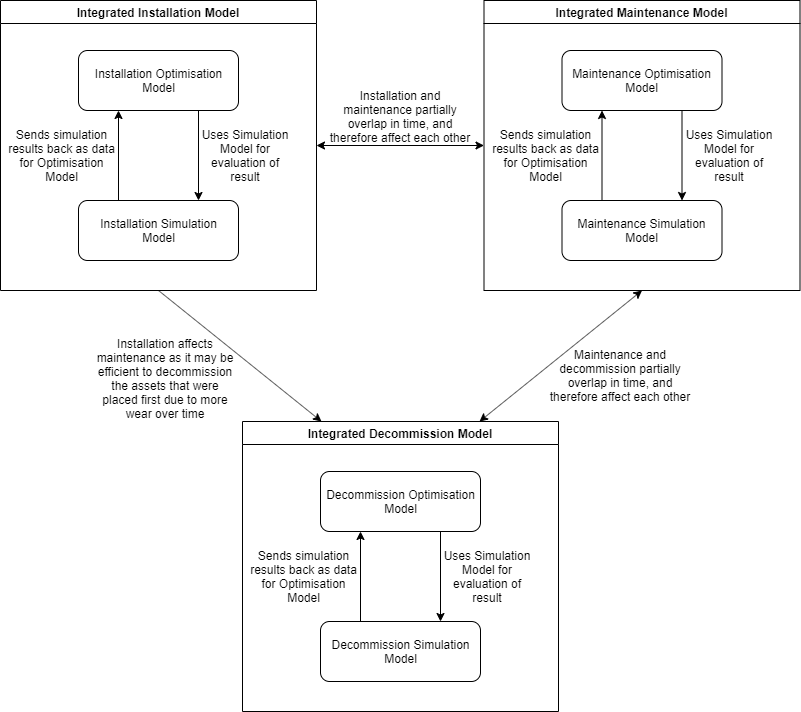
\includegraphics[width = \textwidth]{OWF Tool interactions}
\caption{The connections between each of the minor models that together make up the final model}
\label{f:interact}
\end{figure}

I first plan to start of with simplistic models spanning two or three phases, which can be refined throughout the research. That way details can be added where needed, and the models would be suited to answer the research questions from early on. However I do have some ideas about the models for each phase, and which aspects should be incoporated. These ideas are based on models from the literature, as I am not planning to design completely novel models for the individual phases and instead focus on their interaction and overlap. 

I will now first talk about my goals for the individual models, after which I will talk about their combination and my plans to answer each of the research questions. 

\subsubsection{Models for each phase} \label{sss:phases}
The installation model would effectively be a combination of the two models discussed in \Cref{ss:sched}. In that section I took two focus papers \cite{barlow2018mixed,kerkhove2017optimised} and discussed strengths and weaknesses of both. My hope is to make a hybrid of these two approaches and highlight their strengths. Both approaches used both simulation and optimisation together. I aim to do the same in the manner outlined in \Cref{ss:simopt}, using simulation to evaluate schedules generated by the optimisation model. 

For this, a focus on cashflows also seems to be a good approach, including positive cashflows from partial completion. These will be used together with milestone deadlines. Start date and non-operational periods will both be explored. For this, a dedicated heuristic, as in one of the papers, could be used as a base solution, which can then potentially be improved with a local search. These high-level optimisations will be followed by more detailed ones. For each time period a set of desired vessels should be determined, based on the costs of (de)commissioning and the timespan restrictions on it. Then all tasks will be assigned to a vessel, and for each vessel a schedule will be made. Finally, these detailed schedules will be tested using the simulation model, implemented by the tool described in \Cref{s:sim}. This will check feasibility and quality of the schedule, after which the optimisations can be tweaked based on the findings. This process will repeat for a number of iterations or until a certain quality is reached. 

These are a lot of optimisations that all rely on each other. For that reason it may be computationally heavy. I realize that potentially simplifications need to be made to make this sort of model feasible. If that is the case, there are various possible ways to do that, which will be investigated further if needed. However, as I aim to investigate how the different phases affect each other, the models for the individual phases need to have sufficient detail for possible improvements to be effective and noticeable. 

\bigskip

My plans for the maintenance model are worked out less than those for the installation model. The reason for this is, as previously mentioned in \Cref{ss:maint}, there is yet more reading to be done regarding the maintenance phase. However, with the large amount of research done in this area I am confident I can find some previously used models to base my own models on. As with the installation model, I aim to have optimisation and simulation work together, as shown in \Cref{f:interact}.

Generally the typical subjects in maintenance such as supply chain management and minimising asset failure are significantly more difficult in our context, as there is a large lead up time before any emergency operations can be performed on the site. Intuitively the OSPs are the most vital to prevent failure in, as a failure in one of them can mean dozens of WTGs are no longer producing energy. Therefore I am planning on experiments with various maintenance strategies with the aim of maximising overall profit. As for methods, some form of optimisation will be combined with simulation, as I aim to do for the other phases. For more detail more research will need to be done first, which I will do in the upcoming months.  It is clear there is a relatively large amount of research on maintenance of offshore sites (as compared to a small amount of research on their installation), so any future research will have to build on that.

\bigskip

For the decommission phase there is much less literature than for the other two phases, which means there is no good model from the literature to base my model on.
For that reason I am planning for the decommission model to be similar in structure to that created for installation phase, and the methods should therefore be similar as well. However, the restrictions may be fairly different. Cost-effectiveness is still important, but there may be many more hard restrictions based on government regulations. These will be the restrictions to ensure the project is completed before a certain deadline, as otherwise a later start for the decommission might be more cost-effective. Therefore these projects will hold their own difficulties and are significantly different from installation projects. 

\bigskip

However, as stated before, the above plans are as goals for the individual phases of a life-cycle spanning model. This model will start of very simple, and these goals will slowly be incorporated into it. It is therefore possible that some of the goals here will not be feasible in the final model. Which aspects are feasible and which are not is hard to say at this point, as this is novel research and there is no precedent for designing a model that spans the entire life-cycle. This difficulty is why the choice was made to start off without much detail, and build from there, instead of making detailed models for each of the phases and then combine them. The combination is the part I want to focus on, and should therefore be my starting point. 

\subsubsection{Research questions} \label{sss:questions}
I will now go back through the questions first discussed in \Cref{ss:objs} and give a bit more context for each of them, as well as my plans on how to start answering them. 

\sqa*

These interactions will occur when two phases of the life-cycle partially take place at the same time, namely installation and maintenance at the start, and maintenance and decommission at the end. To fully explore this interaction between installation and maintenance, we need to know which types of vessels can be used for installation tasks, which for maintenance tasks, and which for both. The extend to which exploring this interaction can lead to higher efficiency is determined by how many of the vessels can be used for both type of task. For example a vessel specialised in cable-laying will not be much use for maintenance tasks if cables do not need much maintenance. But a transport vessel might be suited to transport assets for both installation and maintenance operations. The same sort of question needs to be answered when looking at the interaction between maintenance and decommission. 

In order to optimise with this interaction in mind, a model where the fleet compostion and start and end dates of vessel rentals are decision variables might work well. In practice there are minimum periods for vessel rental, and minimum periods for which a vessel can be decommissioned for. There are also costs associated with this. For that reason, optimising these values, and then assigning the available vessels to tasks related to either of the active phases might be a good approach, and will be one of the things I aim to try early on.

\sqb*

This question primarily regards the decomission phase, though maintenance is also affected. In order to optimially decide how to do maintenance we need to use all available information to predict how likely each asset is to fail. Therefore individual histories of each asset should be kept, including when it became active, and any previous failures and repairs. Using this to create a more accurate prediction of failure rates can help in the maintenance phase, but it can also help determine which assets to decomission first. If we predict an asset is likely to fail soon, we ought to decomission that before an asset that will probably continue functioning for a while. This ordering is the primary question in the decomission phase, and I hope to help answer it with my research.

The difficulty in answering this question comes from its reliance on data. I have an intuition that looking at all events in a 20 or 30 year lifespans of many WTGs will reveal some pattern allowing for reasonably accurate predictions on the failure rate, but without having large amounts of data to base models on, and then actual windfarms to test the model predictions with, I cannot say anything conclusive about this intuition. Therefore the first step in attempting to answer this question is gathering as much data as there is available, and then look for patterns in their history of failure. 

\sqc*

This question explores the same general phenomenon as \Cref{sqb} but from the opposite perspective. It therefore primarily influences installation and the early maintenance phase, and even decisions before the installation phase like the layout of the site. In windfarms currently being build the main factor used to decide layout it maximising energy output by minimising wake, the effect that having turbines close together reduces individual output per turbine. However the layout may also affect the failure rate of turbines, and if a minimal reduction in energy output increases uptime this change might be worth it. In the same way, the order the turbines are installed can be done in a way that maximisus energy output, or minimises installation cost, or minimises failure rate and with it maintenance cost. All of these factors need to be weighed to get the optimal solution, and in order to completely measure the maintenance cost we need to look at maintenance throughout the entire life cycle. 

As with \Cref{sqb} this question has a strong reliance on data. In addition to what I've written about that before, there are some extra steps I can take with this question. While there is still reliance on data, if I develop a simulation model for the entire life-cycle I can simply start experimenting to see if early decisions have a long term effect that should be taken into account. As far as I can tell no research has looked at this before, and potentially even a simulation model that is not based on that large amount of data described before is able to find long term impacts of early decisions that are as of yet unknown. 

\rquest*

After the Sub-Questions have been answered some of the major ways phases of the life-cycle can interact with each other will have been explored, and I will then be able to adequately answer this primary question. 

\subsection{Timeline and next steps} \label{ss:timel}
%Timeline and focus from here
Since research is inherently exploratory and unpredictable, it is impossible to have a timeline set in stone. However, in this section I will sketch a possible timeline and outline what I will focus on from here, based on the previously mentioned directions. Note that this timeline is subject to change, especially the further into the future it predicts. 

\bigskip

There are three immediate steps to be taken to start off the research. A simplistic model of multiple phases needs to be made, to then be refined throughout the project. Initially I will start off with a simple model with the installation and maintenance phases included, which can then be tested on a small fictional windfarm. The next step is including the decommission phase, and then iteratively add in details and refinements into the model. Which details will be added in, and in which order, depends on feasibility and how connected they are to the research questions outlined in the previous section. An exact plan can not be given until further on in the process. 

The second step to be taken as soon as possible is starting data collection. My supervisors have worked extensively in this field, and I hope to get in contact with related companies and researchers to gather my data through them. Setting up this connection is important to do early on, as there can in practice be long waiting times before data can be gathered, and if it turns out to be difficult to acquire data alternative options need to be explored rapidly as well. In case some data can be acquired but it is not enough, the available data can potentially be used to generate realistic fictional data. Alternatively if no real data can be acquired I can potentially try to acquire a fictional data set that is close enough to real data to be useful. If none of these options are available, some strong assumptions will need to be made to answer some of these research questions, but this is a last resort, and hopefully at least some data is available. 

The third step which is to be taken rapidly is to read more of the research regarding maintenance projects. At this point in time I have enough knowledge about it to work on the basic model I aim to start off with, but in order to make the appropriate refinements more literature needs to be read. I have however collected a large amount of research in this area, hence the amount of available research will not be a problem here. 

\bigskip

Those are the immediate steps to be taken, and will be where my focus will lie for the next 3 months or so. After that, there will be a time where the main focus lies on improving the models and making them suited to answer the research questions. Determining how long this will take is difficult, as this is an area of research that I am not very familiar with and is unpredictable in nature. However if I had to give a timeframe, I would say I will spend a 6-8 month period primarily focused on model design, implementation, and verification. Secondary tasks in this time are data analysis (or generation, based on the availability of data as discussed above) and early writing. 

Finally the rest of the project will mainly be spend on analysing the results and findings, and writing it all up. The time that will take is again hard to determine, and the time it took to write this report was significantly longer than expected. However in many projects it tends to be that the start is the hardest, so I have some confidence writing up the final thesis will go smoothly. 

Apart from these primary areas of focus, some extra things outside the main research path might crop up. For example, I am looking into more courses and conferences to attend, and potentally some early findings might be written up in a seperate paper. These things will not be a primary focus, but depending on the research progress time may be made for them. 

\pagebreak

\bibliographystyle{agsm}
\bibliography{mybib}

\end{document}